\chapter{Implementasi dan Pengujian}
\label{chap:Implementasi}

Pada bab ini akan ditunjukkan tampilan dari implementasi perangkat lunak dan juga bagaimana perangkat lunak diimplementasikan. Pengujian juga akan diterapkan pada perangkat lunak secara fungsional dan eksperimental. Hasil dari pegujian akan dijelaskan secara rinci dan sistemasi serta akan dibuat kesimpulan untuk pengujian yang telah dilakukan.

\section{Implementasi Antarmuka}
\label{sec:implementasi-antarmuka}

Antarmuka perangkat lunak diimplementasikan dengan memakai \textit{framework} antarmuka grafis berbasis bahasa pemograman Python yang bernama Kivy\footnote{https://kivy.org/\#home}. Implementasi antarmuka disesuaikan dengan rancangan antarmuka perangkat lunak yang telah dibuat pada bab \ref{chap:perancangan}. Berikut ini adalah tampilan antarmuka dari implementasi perangkat lunak.

\begin{figure}
	\centering
	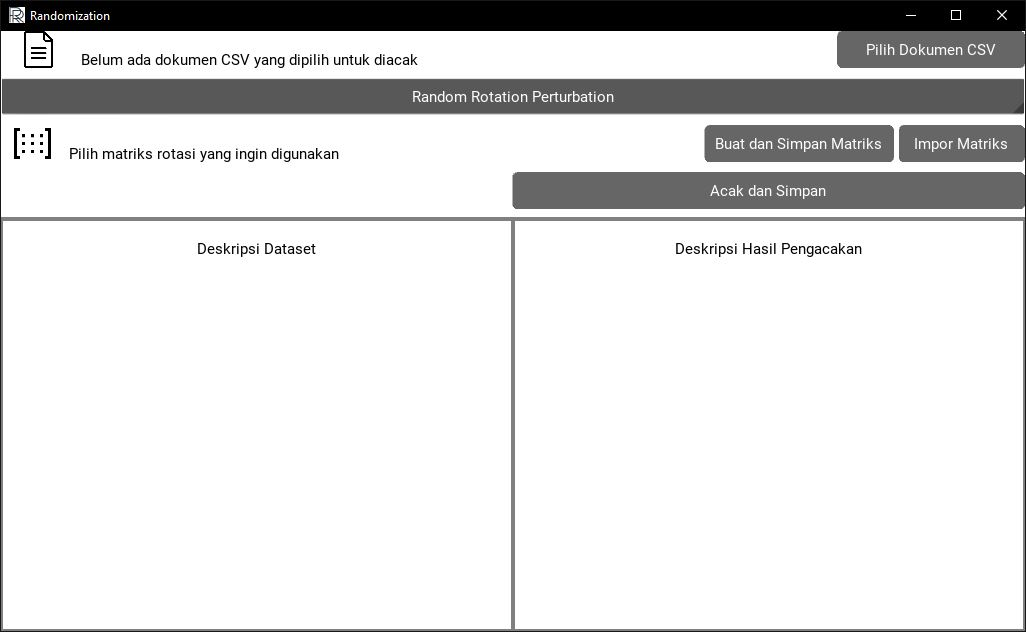
\includegraphics[scale=0.6]{antarmukautama}
	\caption{Tampilan perangkat lunak yang pertama ditampilkan saat perangkat lunak baru dibuka}
	\label{fig:antarmukautama}
\end{figure}

Antarmuka perangkat lunak mempunyai tiga buah bagian yang mempunyai fungsinya masing-masing. Pertama adalah bagian masukan dan pengaturan, terdapat pada bagian atas yang bernomor satu dan dikelilingi kotak merah. Kedua adalah bagian deskripsi dataset, terdapat pada bagian bawah sebelah kiri yang bernomor dua dan dikelilingi kotak biru. Terakhir adalah bagian deskripsi hasil randomisasi, terdapat pada bagian bawah sebelah kanan yang bernomor tiga dan dikelilingi kotak hijau. Ketiga bagian ini akan dijelaskan secara rinci pada subbab-subbab berikutnya.

Perangkat lunak randomisasi ini mengimplementasikan dua buah teknik randomisasi yang berbeda yaitu \textit{Random Rotation Perturbation} dan \textit{Random Projection Perturbation}. Oleh karena itu, antarmuka perangkat lunak akan menyesuaikan dengan teknik yang dipilih oleh pengguna. Ketiga bagian antarmuka yang telah disebutkan tadi dengan otomatis akan berubah sesuai dengan teknik yang dipilih. Pada setiap subbab akan dijelaskan juga sekaligus perbedaan antarmuka teknik randomisasi satu dengan yang lainnya.

\begin{figure}
	\centering
	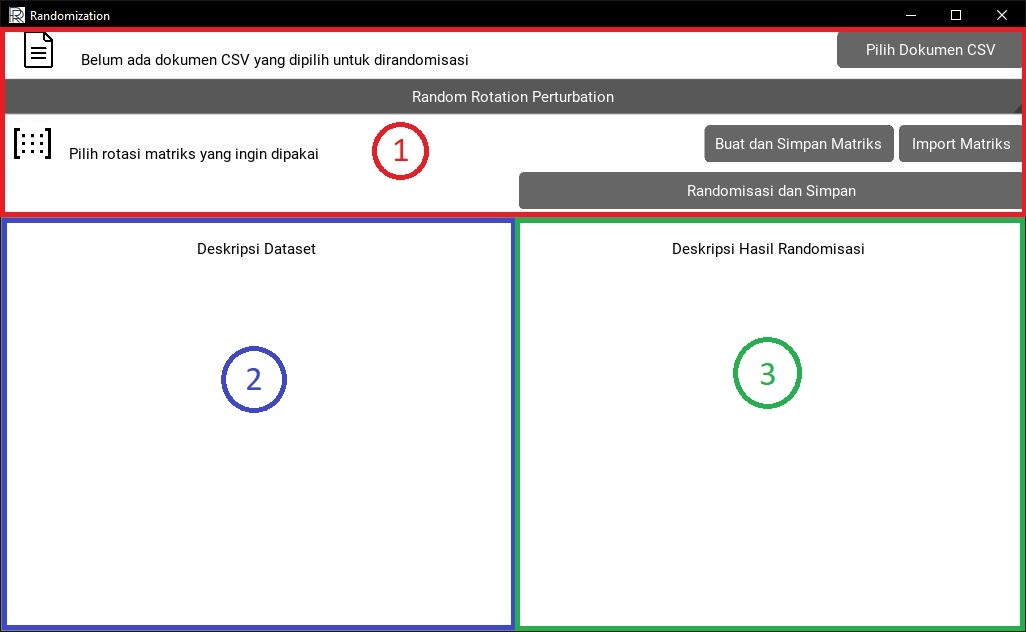
\includegraphics[scale=0.6]{antarmukautamabernomor}
	\caption{Bagian-bagian pada antarmuka perangkat lunak}
	\label{fig:antarmukautamabernomor}
\end{figure}

\subsection{Masukan dan Pengaturan}
\label{sec:masukanpengaturan}

Bagian masukan dan pengaturan menyediakan berbagai interaksi untuk pengguna dapat mengatur masukan yang perlu diberikan kepada perangkat lunak dan menerapkan teknik randomisasi yang diinginkan. Ada beberapa fungsi inti pada bagian ini yaitu masukan dataset berupa file \textit{comma-separated values} yang ingin dirandomisasi, memilih teknik randomisasi yang ingin digunakan, membuat baru dan memilih matriks rotasi atau proyeksi yang ingin digunakan, masukan nilai variabel \textit{epsilon} dan nilai variabel k untuk teknik \textit{Random Projection Perturbation}, dan sebuah tombol untuk menerapkan teknik randomisasi dan menyimpan hasilnya. Berikut akan dijelaskan secara rinci dengan gambar setiap fungsi tersebut dan cara pemakaiannya yang benar secara berturut.

Berikut akan dijelaskan setiap fungsi pada bagian masukan dan pengaturan sekaligus menjelakan cara pemakaian bagian antarmuka perangkat lunak ini. Angka pada gambar   akan sesuai dengan nomor urutan berikut.
\begin{enumerate}
    \item abc
\end{enumerate}

\begin{figure}
	\centering
	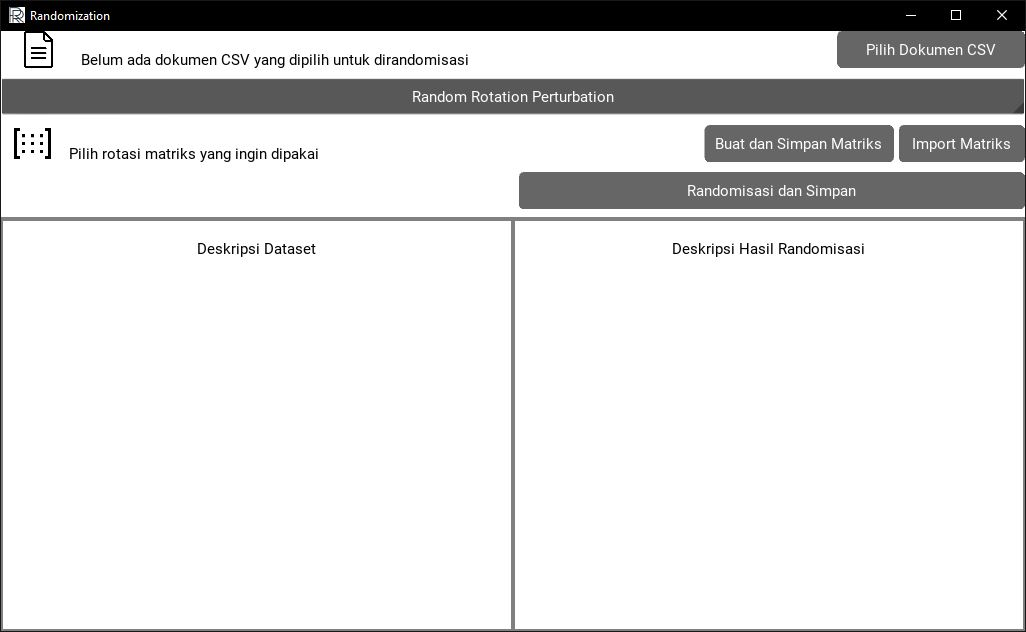
\includegraphics[scale=0.6]{panduanantarmuka}
	\caption{Bagian-bagian pada antarmuka perangkat lunak}
	\label{fig:panduanantarmuka}
\end{figure}


\subsection{Deskripsi Dataset}
\label{sec:deskripsidataset}

\subsection{Deskripsi Hasil Randomisasi}
\label{sec:masukanpengaturan}



\section{Pengujian Perangkat Lunak}
\label{sec:pengujianpl}

\subsection{Pengujian Fungsional}
\label{sec:pengujianfungsional}

\subsection{Pengujian Eksperimental}
\label{sec:pengujianeksperimental}